\begin{figure}[H]
\centering
\includegraphics[page=4,width=0.45\textwidth]{\FCNCFigures/tthML/showFake/faketau/prefit/NOMINAL/reg1l1tau2b2j_ss_vetobtagwp70_highmet/tau_pt_0.pdf}
\put(-100, 140){\textbf{(a)}}
\put(-75, 140){\footnotesize{$W$-jet fake}}
\includegraphics[page=4,width=0.45\textwidth]{\FCNCFigures/tthML/showFake/faketau/prefit/NOMINAL/reg1l1tau2b2j_ss_vetobtagwp70_highmet/mtaujmin.pdf}
\put(-110, 140){\textbf{(b)}}
\put(-75, 140){\footnotesize{$W$-jet fake}}\\
\includegraphics[page=6,width=0.45\textwidth]{\FCNCFigures/tthML/showFake/faketau/prefit/NOMINAL/reg2l1tau1bnj_vetobtagwp70_highmet/tau_pt_0.pdf}
\put(-100, 140){\textbf{(c)}}
\put(-75, 140){\footnotesize{b-jet fake}}
\includegraphics[page=2,width=0.45\textwidth]{\FCNCFigures/tthML/showFake/faketau/prefit/NOMINAL/reg2l1tau2bnj_vetobtagwp70_highmet/tau_pt_0.pdf}
\put(-110, 140){\textbf{(d)}}
\put(-75, 140){\footnotesize{Radiation fake}}\\
%\includegraphics[width=0.45\textwidth]{\FCNCFigures/thq1l2tau/Plots_h1l2tau_Ltauosfakeorig_thuguth.pdf}
%\put(-100, 97){\textbf{(e)}}
%\put(-75, 97){\footnotesize{$l+hh$ OS}}
%\includegraphics[width=0.45\textwidth]{\FCNCFigures/thq1l2tau/Plots_h1l2tau_Ltaussfakeorig_thuguth.pdf}
%\put(-100, 97){\textbf{(f)}}
%waiting for 140 result or removed from the note.
%\put(-75, 97){\footnotesize{$l+hh$ SS}}\\
\caption{ The origins of fake $\tau$'s in the top fake MC for W-jet fake control region (a,b), b-jet fake control region (c), radiation control region (d)%; in the leptonic OS (e) and SS (f) categories.
The flavor distributions are quite similar between OS and SS.}
\label{fig:lh_fake_comp}
\end{figure}

